\chapter{Marco teórico}
\label{ch:marco teorico}

En este capítulo se introducirá y discutirá el trabajo previo realizado y los conceptos necesarios para comprender las distintas técnicas y enfoques utilizados para la construcción de un módelo de predicción de demanda y maximización de ingresos así como el impacto que los resultados tienen dentro de la industria hotelera. Se dará una breve explicación del proceso de gestión de una propiedad mencionando cuales son los principales indicadores de control del proceso, así como las variables estudiadas para la toma de decisiones.

\section*{Gestion de una propiedad}

El proceso de gestión de propiedades o de hoteles comprende una serie de actividades que tienen como objetivo el garantizar la rentabilidad de un proyecto de arrendamiento. Dentro de las actividades que se llevan a cabo están las siguientes:
\begin{itemize}
  \item Gestión de \emph{canales de venta}
  \item Gestión de \emph{segmentos de mercado}
  \item Gestión de \emph{precios por tarifa}
  \item Análisis del \emph{comportamiento de la plaza}
  \item Análisis de \emph{indicadores principales}
\end{itemize}

A continuación profundizaremos en cada una de las actividades que forman parte de este proceso.

\subsection*{Gestión de canales de venta}

El equipo administrativo del hotel o propiedad, deben analizar diariamente el comportamiento de sus canales de venta o distribución. Típicamente un hotel tiene un catálogo estándar de canales de distribución:
\begin{itemize}
  \item Sitio Web 
  \item Call Center / FrontDesk
  \item Agencias de viajes en línea
  \item Globalizadores ~ Agencias de viajes
\end{itemize}

Cada uno de los canales de venta van dirigidos a un segmento de mercado en específico y lo que el equipo de administración debe hacer es asegurar que la demanda del hotel se mantenga lo suficientemente alta para poder asegurar la continuidad operativa del negocio. Para lograr esto se genera una estrategia de distribución, en la cuál se designa parte del inventario a cada uno de los canales y se fija un precio a cada una de las tarifas a ofertar. Los precios para un producto en específico tienden a variar entre los diferentes canales y esto tiene que ver con el costo asociado a la operación de cada uno de los canales. Por ejemplo, el sitio web típicamente es un canal de reservación propio del hotel, lo que significa que las ventas generadas por este canal son libres de comisiones; por el contrario, las agencias de viajes en línea tienden a cobrar una comisión por la venta generada por esos canales.

Lo que la administración del hotel debe conseguir es poder tener la mezcla de ventas entre sus canales que maximice el ingreso, de tal forma que los costos generados por las ventas no \emph{canibalicen} las ganancias de la propiedad. Es con esta restricción donde se descartaría una asignación total del inventario a las agencias de viajes en línea, ya que la comisión de este canal puede ser de hasta el 25\% del total de la venta, lo cual podría representar una pérdida de hasta $\frac{1}{4}$ de las ganancias que se pudieron haber obtenido. Si por el contrario asignaramos todo el inventario disponible a los canales propios del hotel, si bien no se paga una comisión, la demanda generada por estos canales es inferior a la demanda generada por las agencias de viajes en línea.

\subsection*{Gestión de segmentos de mercado}

La gestión de los segmentos de mercado es similar a la gestión de los canales de venta ya que estos estan relacionados a los canales de distribución. 

Las propiedades típicamente distinguen segmentan a sus clientes en las siguientes categorías:

\begin{itemize}
  \item \emph{Clientes directos:} Aquellos clientes que reservan en algún canal directo del hotel
  \item \emph{Clientes de negocios:} Aquellos clientes que pertenecen a una empresa que tiene alguna tarifa convenida con el hotel. Típicamente esta tarifa esta sujeta a una producción de cuartos durante un periodo
  \item \emph{Clientes de mayoreo:} Aquellos clientes que reservan utilizando un canal mayorista; puede ser una agencia de viajes en línea o mediante un agente de viajes.
  \item \emph{Grupos:} Aquellos clientes que llegan a la propiedad como parte de un grupo.
\end{itemize}

Para gestionar eficientemente los segmentos de mercado se debe crear una estrategia de asignación de precios a las diferentes tarifas que van dirigidas a cada uno de ellos. Por ejemplo, un \emph{cliente directo} que llega al hotel sin reservación, es propenso a pagar un precio mas alto por una habitación disponible, al contrario de un cliente que viene como parte de un grupo que reservó con mayor tiempo de anticipación con una tarifa mucho mas baja. El equipo administrativ\emph{}o debe cuidar los segmentos de mercado que ocupan la propiedad ya que el tener un grupo muy grande ocupándola significa muchas veces tener un hotel lleno a una tarifa muy baja y con mayor desgaste en las habitaciones, y por el otro lado, no siempre es posible llenar un hotel con clientes que llegan sin reservación los cuales están dispuestos a comprar una habitación a un precio mas elevado.

\subsection*{Gestión de precios por tarifa}

Una de las actividades mas importantes del proceso de gestión de una propiedad es la gestión de los precios por tarifa ya que generalmente las tarifas disponibles en un hotel están asociadas a un segmento de mercado y a un canal de reservación. Para poder realizar esta actividad se debe establecer una estrategia en la cual se define si se quiere incrementar la ocupación de la propiedad o si se quiere incrementar el \emph{RevPAR}(revenue per available room). Una vez establecida la estrategia inicial se deben modificar los precios para las tarifas que impactan los canales y segmentos donde se quiere fomentar la demanda o incrementar el precio. Si el objetivo es el primero, lo mas probable es que el cambio emplique una baja en las tarifas o creación de promociones sujetas a diversas restricciones, en cambio, si el objetivo es el segundo muy probablemente el cambio implique una alza en algunas tarifas y el cierre de algunas tarifas en donde este incremento no se pueda llevar a cabo por temas contractuales, por ejemplo las tarifas convenidas con otras empresas o clientes.

Es importante mencionar que la ejecución de esta tarea dentro del proceso de gestión depende del análisis continuo de la información histórica generada por el hotel (comportamiento de la propiedad en años anteriores en la misma fecha sujeta al estudio), conocimiento de la plaza en donde se ubica la propiedad (depende de la experiencia del equipo administrativo del hotel), información ajena al hotel (situación marco económica, eventos cercanos a la plaza, desempeño de la competencia cercana a la propiedad, etc). Muchas veces el conocer esta información implica un gran esfuerzo por parte del equipo ya que la información tiende a estar distribuída en diversos sistemas o en ocasiones deberán recabarla físicamente (visitando a su competencia o haciendo llamadas telefónicas) dejando un riesgo latente de recibir información que no es precisa.

Otra de las fuertes dependencias para la ejecución efectiva de esta tarea es contar con sistemas que distribuyan los nuevos precios en todos los canales disponibles en poco tiempo y con poco esfuerzo ya que de lo contrario no tendria sentido realizar esta labor si al final los precios no pueden ser cambiados dentro de un tiempo en el que el mercado pueda responder de acuerdo a lo planeado durante el análisis de la información. Una vez que los precios son alterados, el equipo deberá analizar nuevamente la información para asegurar que los cambios tuvieron los efectos deseados, de lo contrario, se deberá cambiar la estrategia lo antes posible para evitar afectar el desempeño de la propiedad.

\subsection*{Análisis del comportamiento de la plaza}

En el sector de la hotelería en México, se le llama plaza a la ubicación geográfica en dónde se encuentra una propiedad y típicamente agrupa a propiedades independientes o de otras marcas (set competitivo), oficinas, corporativos, centros comerciales, y lugares de interés turístico. La plaza genera gran cantidad de información que es de interés para el equipo administrativo de una propiedad, ya que el desempeño financiero de esta depende mucho de la situación que presenta la plaza en un momento determinado.

Los hoteles que comparten una plaza generalmente están dispuestos a compartir información de su propiedad con otros, de esa forma pueden tener un conocimiento mas amplio sobre la realidad que se vive en ella. Si una propiedad requiere obtener datos de su competencia, basta con una simple llamada telefónica a la propiedad de interés para solicitar los datos de interés, por ejemplo: \emph{cuartos ocupados}, \emph{cuartos disponibles}, \emph{cuartos fuera de servicio}, \emph{ingresos generados por la venta de habitaciones}. Con esta información se pueden calcular algunos indicadores que son indispensables para el an{alisis del comportamiento de la plaza:
\begin{itemize}
  \item \% de Ocupación: $\frac{cuartos\ ocupados}{cuartos\ disponibles}$
  \item ADR (Average Daily Rate o Tarifa Promedio): $\frac{ingresos}{cuartos\ ocupados}$
  \item RevPAR (Revenue per available room o Tarifa Efectiva): $\frac{ingresos}{cuartos\ disponibles}$
\end{itemize}

Para poder conocer la situación de una propiedad frente a la competencia en una plaza se generan otros indicadores que facilitan este tipo de análisis.

\begin{itemize}
  \item Penetración de ocupación: $\frac{\%\ ocupacion}{\%\ ocupacion\ plaza}$
  \item Penetración de tarifa: $\frac{tarifa\ promedio}{tarifa promedio\ plaza}$
\end{itemize}

El hotel o propiedad que cuente con los valores mas altos para estos indicadores será el hotel con mayor demanda y mayores ingresos dentro de la plaza, sin embargo, para que el análisis sea efectivo se debe escoger al set competitivo de manera adecuada, de tal forma que los hoteles contenidos dentro de este set sean de la misma gama y vayan dirigidos al mismo público objetivo.


\subsection*{Análisis de indicadores principales}

Como se mencionó anteriormente, existen indicadores de desempeño de una propiedad u hotel que deben ser estudiados de manera diaria para poder tomar decisiones que mejoren el desempeño de esta, asegurando una continuidad operativa y la rentabilidad del inmueble:

\begin{itemize}
  \item \% ocupación
  \item ADR
  \item REvpar
\end{itemize}

Típicamante durante el análisis realizado, se compara el desempeño de cada uno de estos indicadores de manera diaria, mensual y anual, comparando los valores contra el año anterior y buscando siempre una variación positiva entre años. En caso de tener variaciones negativas se debe buscar la causa de esta variación. Se puede tratar de una baja en la demanda general de la plaza, un periodo de recesión financiera generalizada, un nuevo competidor en la plaza, etc. Una vez identificado la causa se deben tomar las acciones necesarias para generar demanda a la propiedad en cuestión. Típicamente la forma más efectiva de hacerlo es modificar los precios de tal forma que el mercado responda favorablemente sin afectar la rentabilidad del inmueble.

\section*{Antecedentes: Modelos de Revenue Management}

Podemos definir la práctica de \emph{revenue management} como la aplicación de técnicas analíticas que intentan predecir el comportamiento de un consumidor al nivel de un micro mercado, optimizando la disponibilidad de productos y sus precios de tal forma que maximicen el crecimiento de los ingresos. El principal objetivo de esta práctica es vender el producto indicado al cliente indicado al tiempo indicado en el precio indicado. La escencia de esta práctica radica en entender la percepción del producto que tienen los clientes y alinear los precios de estos productos de acuerdo a esta haciendo una correcta segmentación de los clientes objetivos.

Es importante mencionar que la disciplina de \emph{revenue management} se compone de dos partes principales:
\begin{enumerate}
  \item Pronóstico de ocupación
  \item Asignación de precios
\end{enumerate}

En las siguientes secciones discutiremos acerca de los trabajos previos sobre los dos principales componentes de esta disciplina.

\subsection*{Trabajo previo: modelos de pronóstico de ocupación}

La base de una práctica efectiva de \emph{revenue management} es un buen modelo de pronóstico de demanda, ya que el resultado de este será la entrada del modelo de optimización de precio de tal suerte que mientras menor sea el error en el pronóstico de la demanda, mejor será la optimización de los precios para cada uno de los productos sujetos al análisis.

Se tiene registro de trabajo previo para el desarrollo de modelos de pronóstico de demanda en diferentes industrias, algunas de ellas son: \emph{líneas aéreas}, \emph{retail}, \emph{telecomunicaciones} y \emph{hospitalidad}, siendo la primera la que cuenta con modelos de pronóstico más maduros, este hecho obedece a que en esta industria es en dónde a principios de los años 80's nace la disciplina de \emph{revenue management}. 

La venta de asientos en un vuelo es un caso dónde naturalmente se puede utilizar un modelo de optimización de ingresos ya que cuenta con ciertas características que hacen que el modelado del problema sea muy intuitivo:
\begin{itemize}
  \item Se cuenta con un inventario reducido
  \item El inventario es perecedero (una vez que el avión despega, los asientos vacíos no generan un ingreso
  \item Se cuenta con un amplio segmento de mercado que genera demanda sobre el producto
  \item Los asientos se compran con distintos tiempos de anticipación (hay clientes que compran con un mayor tiempo de anticipación que otros)
  \item Se conoce el tiempo de estancia de cada uno de los clientes en la aeronave.
\end{itemize}

Las condiciones mencionadas anteriormente facilitan la construcción de un modelo de pronóstico de demanda. A continuación haremos una breve descripción de la evolución de este tipo de modelos a lo largo del tiempo.

\texttt{Beckmann y Bobkowski (1958)} presentaron modelos estadísticos que describen reservaciones de pasajeros, cancelación de reservaciones y \emph{no shows}. En su trabajo los autores comparan modelos utilizando diferentes distribuciones probabilísticas: \emph{Poisson}, \emph{Binomial Negativa} y \emph{Gamma} aplicadas en datos generados por aerolineas con la finalidad de modelar las reservaciones efectivas y propone una condicion optima para un nivel de sobreventa para un vuelo en partícular.

Posteriormente, otros autores continuaron explorando nuevas metodologías para poder construír modelos de predicción de demanda. Uno de los autores mas citados en las investigaciones de modelos de pronóstico de demanda es Lee (1990) que presenta un artículo en donde explica don enfoques para resolver el problema de pronóstico de ocupación en aerolíneas:
\begin{itemize}
  \item Modelos de series de tiempo 
  \item Modelos basados en información de reservaciones
\end{itemize}

Los modelos basados en series de tiempo consideran unicamente las series de tiempo con la información de llegadas o porcentajes de ocupación aplicandoles modelos de series de tiempo (como suavizamiento exponencial, ARIMA, etc). En estos casos no se utiliza la información propia de las reservaciones.

El enfoque basado en reservaciones hace uso de la información contenida en las reservaciones para pronosticar llegadas futuras. En este tipo de modelos típicamente se considera el concepto de \emph{pick-up}. Esto quiere decir que dadas \emph{K} reservaciones para un dia futuro \emph{T}, esperamos tener un \emph{pick-up} de \emph{N} reservaciones más desde este momento hasta el momento T. El pronóstico entonces será \emph{K + N}

Existen dos versiones del modelo de \emph{pick-up} (\texttt{Weatherford y Kimes}, 2003). La versión aditiva del modelo en donde a las reservaciones registradas en el hotel se le suman el promedio de reservaciones que típicamente llegan en un periodo entre la fecha actual y la fecha de llegada del huésped (tomando la temporalidad del hotel en cuenta), y la versión multiplicativa, la cual es muy similar, con la única diferencia de únicamente se toma en cuenta una fracción de las reservaciones actualmente registradas en el hotel.

Existen trabajos en los cuales se presenta un modelo avanzado en el cual se combinan modelos de series de tiempo y modelos basados en reservaciones, tal es el caso del artículo presentado por \texttt{Flides y Ord} (2002) en el cuál se concluye que la combinación de ambos modelos generalmente tienen un mejor desempeño en cuanto al pronóstico de la demanda. Otro trabajo que presenta un enfoque similar es el realizado por \texttt{Sa} (1987) en el cuál se utiliza una regresión multiple para desarrollar un modelo de pronóstico combinado, en este caso, la variable dependiente eran las reservaciones pendientes por llegar mientras la variable independiente incluía el número de resrvaciones confirmadas, un índice de temporalidad,  índice semanal y un promedio del comportamiento histórico de las reservaciones pendientes. Esta regresión se corría para varios días antes de la llegada de los clientes (t = 7, 14, 21, y 28).

Es importante hacer las siguientes observaciones sobre los modelos comentados anteriormente:

\begin{itemize}
  \item Los modelos de regesión lineal asumen que existe una correlación entre el número de reservaciones confirmadas y el número final de reservaciones (en el día 0), de tal forma que: $pronostico_{dia0} = a + b * reservaciones_{diaN}$
  \item Los modelos de regresión logarítmica asumen que existe una correlación entre el número de reservaciones confirmadas y el número final de reservaciones (en el día 0), de tal forma que: $log(pronostico_{dia0} = a + b * log(reservaciones_{diaN}$
  \item El modelo aditivo suma las reservaciones actuales al promedio histórico del \emph{pickup} de reservas desde el día de la lectura \emph{diaN} hasta el dia de la estancia \emph{dia0}: $pronostico_{dia0} = reservas_{diaN} + \sum_{i=0}^{n} \frac{pickup_i}{n}$
  \item El modelo multiplicativo multiplica las reservaciones actuales por la proporción del promedio histórico de reservaciones  desde el \emph{diaN} hasta el dia de la estancia \emph{dia0}: $pronostico_{dia0} = reservas_{diaN} * \frac{reservas_n - \sum_{i=0}^{n} \frac{pickup_i}{n}}{reservas_n}$
\end{itemize}

La tabla 2.1 resume los modelos más comunes utilizados para pronosticar ocupación, agrupados por categoría.


\begin{table}[]
\centering
\begin{tabular}{|c|l|}
\hline
\multicolumn{1}{|l|}{Categoria} & Modelo                                                                                                                                                    \\ \hline
Historico                       & \begin{tabular}[c]{@{}l@{}}1. Mismo día año anterior\\ 2. Promedios móviles\\ 3. Suvizamiento exponencial\\ 4. ARIMA\end{tabular}                         \\ \hline
Avanzado                        & \begin{tabular}[c]{@{}l@{}}1. Aditivo\\   a. Pickup Clasico\\   b. Pickup Avanzado\\ 2. Multiplicativo\\   a. Curva de reservaciones\end{tabular}         \\ \hline
Combinados                      & \begin{tabular}[c]{@{}l@{}}1. Promedios ponderados de modelo histórico y modelo avanzado\\ 2. Regresión \\ 3. Modelo de información completa\end{tabular} \\ \hline
\end{tabular}
\caption{Modelos de pronosótico por categoría}
\label{ModelosOcup}
\end{table}

\subsection*{Desempeño de modelos de pronóstico}

Se han realizado estudios con el objetivo de comparar el desempeño de los modelos previamente presentados, a continuación presentaremos los resultados obtenidos.

\texttt{Wickham} (1995) estudió la efectividad de una variedad de modelos de pronóstico de ocupación utilizando datos de aerolíneas. Durante este trabajo se comparan modelos históricos de ocupación (utilizando promedios simples y promedios ponderados) y modelos de \emph{pickup} (clasicos y avanzados) llegando a la conclusión de que los segundos son más efectivos, al menos para los datos aplicados durante su análisis.

\texttt{Weahterford} (1998) comparó los modelos aditivos frente a los modelos multiplicativos y modelos de regresión dentro del contexto de las aerolíneas y encontró que los modelos aditivos y de regresión tienen un mejor desempeño que los multiplicativos.

\subsection*{Modelos de machine learning}

Si bien las técnicas estadísticas anteriormente mencionadas pueden predecir efectivamente níveles de ocupación y demanda, se requieren de amplios conocimientos en estadística y de largos procedimientos para poderlas aplicar de manera tal que funcionen correctamente o de otra manera se puede optar por el uso de \emph{software} comercial el cuál resulta muy costoso la mayoría de las veces. Para solventar estos hechos, algunos autores presentan un enfoque diferente para construír modelos de predicción de ocupación, tal es el caso de \texttt{Caicedo-Torres, Payares} (2016) quienes proponen el uso de algorítmos de \emph{Machine Learning} para construír modelos predictivos de ocupación y demanda en la industria de la hospitalidad. La ventaja de estos modelos es que estan listos para ser utilizados por el staff administrativo de la propiedad  sin la necesidad de contar con amplios conocimientos de estadística. Además, estos modelos tienen la ventaja de poder ser empaquetados dentro de aplicaciones de bajo costo, o de ser ejecutados en una infraestructura basada en la nube, lo cual significan soluciones rentables para el sector de hospitalidad.

A continuación presentaremos a detalle algunos algorímtos de \texttt{M.L.} utilizados para la construcción de este tipo de modelos.

\subsubsection*{Regresión de Ridge}

La regresión de ridge es un algorítmo de regresión que incluye un término de regularización en su función de costos con el fin de lograr una mejor aproximación al momento de generalizar el modelo. La regresión de Ridge penaliza el algorítmo con un factor proporcional a la norma Euclidiana (L2) del vector de parámetros. $$J(\theta)=\sum_{i=1}^{n} (\theta^Tx_i - y_i)^2 + \alpha||\theta||^2$$

Dónde el factor de regularización $\alpha$ controla la importancia relativa de la penalidad compleja. Para optimizar esta ecuación se debe encontrar la derivada de la función de costos e igualarla a cero, de tal forma que el vector de parámetros que minimza el error es: $$\theta = (X^TX+\lambda I)^{-1} X^T y$$

Las nuevas predicciones se pueden calcular como sigue: $$h(X) = \theta^Tx=\sum_{i=1}^{n} \theta_ix_i$$

\subsubsection*{Ridge Regresión con Kernel}

Este método consta de aplicar el truco del Kernel a la regresión previamente comentada, esto con la finalidad de projectar los datos originales en un espectro de variables sin tener que explicitamente calcular las transformaciones. Para esto, se comienza con el vector de pesos optimizados para la Regresión de Ridge: $$\theta = (X^TX+\lambda I)^{-1} X^T y$$

Se manipula algebraícamente para obtener: $$\theta = X^T(XX^T + \lambda I)^{-1}y$$

De tal forma que una predicción puede ser obtenida por: $$h(x') = \theta^Tx' = y^T(XX^T + \lambda I)^{-1}Xx'$$

Una función de Kernel evalúa a un producto punto de la forma $$f(x_1,x_2) = \phi (x_1)\cdot \phi (x_2)$$ sin tener que explícitamente calcular la transformación $\phi$. Si definimos $K_{i,j}=f(x_i,x_j)$ y $k_i = f(x_i,x')$, donde $x_i$ es la iésima fila de la matriz $X$, entonces $$h(x') = \theta^Tx' = y^T(K + \lambda I)^{-1}k$$

Ajustamos un modelo en un espacio dimensional mayor inducido pro $\phi$ sin tener que incurrir en una complejidad computacional adicional. Se pueden utilizar varios Kernels, entre los más populares están el Kernel polinomial $$k(x_1,x_2)=( \gamma x_{1}^{T} x_2 + \beta)^ {\delta}$$

Y el Kernel Gaussiano $$k(x_1,x_2)=exp(-\frac{||x_1-x_2||^2}{2{\delta}^2})$$

\subsubsection*{Red neuronal multicapa}

Una red neuronal es un modelo de \texttt{M.L.} capáz de clasificar y realizar regresión. Esta compuesta por $n$ capas totalmente conectadas de neuronas artificiales formando un grafo conectado (en el caso más simple se tiene una capa oculta y una capa de salida). En este modelo, la salida de cada capa de neuronas será la entrada de la siguiente capa. La función de activación es dada por la siguiente ecuación $$y=f(\sum_{i}^{n} w_ix_i+b)$$ donde $f$ es una función de activación. Entre las opciones más populares se encuentran la sigmoide $y = (1+exp(-x))^{-1}$ y la función lineal $y=x$. La elección de la función de activación en la capa de salida define el tipo de red neuronal (si clasifica o realiza regresión)

Las redes neuronales son entrenadas mediante un algorítmo llamado \emph{propagación hacia atrás (backpropagation)} que es una aplicación del algorítmo de descenso por gradiente que toma en cuenta la contribución de las neuronas de la capa oculta al error $E$

\subsubsection*{Red neuronal de base radial}

Las reded nueronales de base radial (RBF) usualmente tienen una sola capa oculta que emplea una serie de funciones llamadas \emph{funciones de base radial} como detectores de características. Las redes RBF pueden ser utilizadas para realizar regresiones o clasificaciones. En este modelo la capa oculta utiliza funcion gaussiana como función de activación $\phi$: $$\phi_j(x)=exp(-\frac{||x-\mu_j||^2}{2\sigma_j^2})$$

Y como función de salida, se tiene la siguiente ecuación: $$y(x)=\sum_{j=0}^{M} w_{kj} \phi_j(x)$$

donde $w_{kj}$ es el vector de pesos que conecta la neurona $j$ de la capa oculta con la neurona $k$ de la capa de salida.

El entrenamiento de este tipo de modelos consiste en encontrar un conjunto de valores para los parámetros $\mu_j$, $\sigma_j$ y $w_{jk}$ que maximizan el desempeño de la red. 

\subsection*{Desempeño de algoritmos de M.L.}

Para realizar el entrenamiento, validación y pruebas de estos modelos se utilizó un proceso de \emph{Cross Validation} en cada uno de los data sets. Los pronósticos se hicieron para un día posterior y para 7 días posteriores, midiendo el desempeño del modelo utilizando la medida \emph{MAPE} (Mean Absolute Percentage Error) definida como: $$MAPE=\frac{1}{n}\sum_{t=1}^{n}|\frac{y_t-h_t}{y_t}|$$

Los resultados mostraron que la \emph{regresión de Ridge} una transformación polinomial de grado dos tuvo el mejor desempeño con un \emph{MAPE} del 8.2012\% durante la validación y un \emph{MAPE} del 8.6561\% durante las pruebas. Durante el proceso de pruebas no se tuvo evidencia de sobreajuste del modelo.

Por otra parte el modelo la \emph{regresión de Ridge con Kernel} tuvo un \emph{MAPE} de 8.69622\% durante la validación, seguido por la \emph{red neuronal} con un \emph{MAPE} del 12.89174\% y finalmente la \emph{red neuronal RBF} con un \emph{MAPE} de 26.32086\%.

Los resultados obtenidos durante esta investigación fueron bastante prometedores sustentando el uso de modelos de \texttt{M.L.} como modelos de caja negra para estimar la ocupación futura de una propiedad, sin requerir conocimiento o experiencia estadística del estaff del hotel, permitiendo nuevos avances el las técnicas de \emph{revenue management} en el sector de hospitalidad.

\subsection*{Modelos de Big Data}

En el sector de turismo y hospitalidad se han hecho esfuerzos para obtener modelos de pronóistico de llegadas y ocupación basados en información generada a partir de las búsquedas en páginas web y el tráfico generado en ellas. Si bien, los resultados obtenidos han confirmado la validéz de algunas fuentes de datos generados en línea, poco trabajo se ha hecho cruzando diferentes fuentes de datos, por ejemplo, utilizar los datos de las búsquedas realizadas en \emph{Google} combinados con el tráfico generado en el sitio web del hotel, los cuales deben estar altamente correlacionados (Tierney y Pan 2012).

Existen algunos trabajos en donde se adoptan dos métodos principales para obtener la ocupación de un hotel a partir de datos generados en línea. Los metódos utilizados son: \emph{Promedios móviles integrados autoregresivos con variables externas} y \emph{Modelo de regresión dinámica con cambios Markov (MS DR)}

En el estudio presentado por \texttt{Pan y Yang (2017)} se presentan dos modelos de series de tiempo en el que se incoroporan tres fuentes de información generada en línea para predecir la ocupación de un hotel. Los datos de entrada contenían datos que describían:
\begin{itemize}
  \item Tráfico generado en el sitio web de la propiedad
  \item Información relacionada con las peticiones realizadas a los motores de búsquedas (\emph{Google})
  \item Información del clima en el destino en dónde se ubica la propiedad
\end{itemize}


El primer modelo presentado es un modelo \emph{ARMAX} en donde se utilizan variables generadas con \emph{big data} como predictores directos de la ocupación. El modelo se definió de la siguiente manera: $$y_t = \alpha + x_t \beta + \mu_t$$ $$\mu_t = \sum_{i=1}^{m} \rho_i \mu_{t-i} + \sum_{j=1}^{n} \theta_j \epsilon_{t-j} + \epsilon_i$$

donde $y_t$ es la variable dependiente y $x_t$ es un vector de variables exógenas independientes. Si $\beta$ es igual a 0, el modelo se convierte en un modelo ARMA(m,n) estándar.

El segundo modelo presentado en este trabajo es el MSDR específicado como: $$y_t = \tau_s + x_t \alpha + z_t \beta_s + \epsilon_s$$

dónde $\tau_s$ es el estado de intercepción; $x_t$ es un vector de variables exógenas con coeficientes independientes del estado; $z_t$ es un vector de variables exógenas con coeficientes dependientes del estado $\beta_s$; $\epsilon_s$ es un error normal \emph{i.i.d} con media 0 y una varianza dependiente del estado de $\sigma^2$.Este modelo permite a las variables en el vector $z_t$ con parámetros dependientes del estado tomar diferentes comportamientos basados en el estado que responden a un proceso de Markov con $J$ estados y una probabilidad transicional $p_{ij}$ específicada como sigue: $$p_{ij} = \frac{1}{1 + \sum_{m=1}^{k} exp(-q_{im})}\ si\ j = k$$ $$p_{ij} = \frac{exp(-q_{ij})}{1 + \sum_{m=1}^{k} exp(-q_{im})}\ si\ j \neq k$$

donde $q_{ij}$ es el parámetro transformado definido como $$q_{ij}=-log(\frac{p_{ij}}{p_{ik}})$$

Para empezar con la estimación del modelo se utiliza el algorimto EM \emph{expectation-maximization} el cuál arroja el valor inicial. Posteriormente se predicen las probabilidades de cada uno de los estados y actualizando la verosimilitud en cada paso. Un paso clave de esta estimación es el cálculo de la verosimilitud de los estados latentes la cual es obtenida mediante la iteración de la verosimilitud condicional.

Para medir el desempeño de ambos modelos se utilizó la medida \emph{MAPE} $$MAPE=\frac{1}{n}\sum_{t=1}^{n}|\frac{y_t-h_t}{y_t}|$$ 

Los resultados arrojan que el modelo ARIMAX tuvo un mejor desempeño con un \emph{MAPE} del 3.804\% comparado con el 4.714\% obtenido por el modelo MS DR

Se puede concluír que los modelos basados en big data presentan una alternativa para poder generar pronósticos de ocupación y demanda utilizando información exógena a los hoteles, sin embargo se debe tomar en cuenta que el costo asociado a la configuración y puesta en marcha de este tipo de modelos es alto ya que se debe de contar con una infraestructura que pueda soportar el manejo de grandes volúmenes de información.


\subsection*{Modelos de optimizacion de ingresos}

Recordemos que un systema de gestión de ingresos para un hotel se puede clasificar dentro de dos grandes grupos (Abdel Aziz et al, 2011). En el primer grupo tendremos todos los sistemas que controlan la cantidad de inventario que se ofrece a cada segmento de cliente. Es decir, se asigna dinámicamente un porcentaje de inventario con un precio fijo distinto para cada uno de los segmentos estudiados por el hotel. El segundo grupo se distingue por asignarle un precio de manera dinámica al inventario que cuenta con características similares. El precio será ajustado continuamente en el tiempo basando los cambios en las variaciones de la oferta y la demanda del producto.

En esta sección se presentaran los módelos utilizados en trabajos anteriores para poder asignar precios dinámicos a un inventario con el fin de maximizar los ingresos de una propiedad.

\subsection*{Modelo de multiplicadores de precio}

El módelo de multiplicadores de precio propone un enfoque sencillo para resolver el problema de maximización de ingresos de una propiedad.

Este modelo propone tener un precio base de referencia (dependiendo de la temporalidad del hotel) y modificarlo utlilizando un conjunto definido de multiplicadores (cuyo valor se encuentra alrededor del 1) y que son infulenciados por variables sensibles a la operación de la propiedad, por ejemplo el \% ocupación, el tiempo de antelación de una reserva, etc., de tal forma que cada multiplicador ajusta el precio por encima o por debajo del precio de referencia. 

El objetivo de este modelo es maximizar los ingresos de la propiedad tomando en cuenta la demanda y la elasticidad del precio. Este modelo tiene la ventaja de enmarcar el pecio en términos de \emph{primas} o \emph{descuentos} en un tiempo variable o sobre un precio de referencia temporal definido por el staff de la propiedad y al ser un modelo muy sencillo de entender permite que el gerente de la propiedad transimita un poco de su experiencia al modelo al ser el quien define el precio de referencia para cada una de las temporadas del hotel.

En trabajos previos se pronponen las siguientes variables que influencían le efecto en los precios:
\begin{itemize}
  \item Tiempo de antelación de una reserva
  \item Habitaciones disponibles al momento de crear una reservación
  \item Tiempo de estancia de una reserva (LoS)
  \item Número de cuartos reservados (tamaño de grupo)
\end{itemize}

A partir de estas variables de influencia se construyen multiplicadores (1 multiplicador por cada variable). Para simplificar la formulación del problema, los multiplicadores usualmente sonn formulados como funciones lineales de las variables de infulencia. Las funciones lineales son elegidas tomando en cuenta una relación lógica entre las variables de influencia y el comportamiento de la propiedad, por ejemplo, si al momento de hacer una reserva hay una alta disponibilidad de habitaciones entonces se esperaría que el multiplicador del precio lo haga bajar con la finalidad de incrementar la demanda de la propiedad.

El modelo recomendará un precio tomando en cuenta el precio de referencia dado por el gerente de la propiedad y los multiplicadores utilizando la siguiente fórmula:

$$Precio_{final} = P_{Referencia} * M_{tiempo} * M_{capacidad} * M_{LoS} * M_{Grupo}$$

Como se puede observar, este modelo es sencillo, sin embargo tiene algunas limitantes:
\begin{itemize}
  \item Las funciones lineales de los multiplicadores deberán ser afinadas continuamente
  \item Todo el modelo depende de la elecciòn de un precio inicial dado
  \item Se debe estimar la elasticidad del precio, esta estimación tendrá un error
\end{itemize}

Sin embargo, una gran ventaja de este modelo es la forma transparente en la que opera, permitiendo que el equipo administrativo de las propiedades se familiarice con estos sistemas.



\subsection*{Modelo de maximización sujeto a restricciones}

Un hotel tipicamente designa un conjunto definido de categorías de precio, posteriormente asigna un inventario a cada categoria, de tal forma que las reservaciones que se hacen con un mayor tiempo de anticipación reciben un precio mas bajo y conforme el inventario se va agotando se reservan las habitaciones con una categoría de precio mayor. El problema con este enfoque radica en que si se asigna un gran número de cuartos a la categoría de precios mas baja, se tendrá un gran número de reservaciones pero a costo de una pérdida en el ingreso generado, y por el contrario, si se asigna un mayor número a la categoría con el precio mas alto se dejaran mas cuartos sin vender.

Este tipo de modelos permite al equipo que administra la propiedad encontrar el precio óptimo para cada categoría en cada noche de tal forma que el ingreso se maximice. Esto conlleva a un sofisticado problema de optimización que tome en cuenta las reservaciones futuras y su probabilidad de ocurrencia. Los precios son dinámicos y cambian día con día. Hay que mencionar que para que este modelo sea certero depende de una buena estimación de la demanda futura de los cuartos.

Para formular el modelo, se define una estancia por los parámetros \emph{(a,L)}, dónde \emph{a} es la primera noche de estancia y \emph{L} es la duración de la estancia, de tal forma que el modelo queda definido como sigue:

Maximizar $$\sum_{l=1}^{Max\ l} P_l O_l$$

Sujeto a $$O_l \leq C_l\  \forall l$$ $$P_l \geq 0 \ \forall l$$

Dónde las variables de decisión del modelo son:

$P_l$: Precio para la noche $l\ \forall l$

Y las variables auxiliares:

$X_{a,L}$: El numero de cuartos asignado a una estancia del tipo $(a,L)$ definido como: $$X_{a,L} = d_{a,L}(\frac{\sum_{l=a}^{a+L-1} P_l}{L*P_{nominal}})^e$$

$O_l$: Es el número de habitaciones reservadas para una noche dada y está definida como sigue $$O_l = \sum_{a,L\in N_l} X_{a,L}$$

Y las entradas del modelo:

$P_{nominal}$: Precio nominal de la propiedad (usualmente la tarifa promedio histórica)

$e$: Elasticidad entre precio y demanda

$d_{a,L}$: La demanda de la estancias tipo $a,L$

$N_l$: El número de estancias que utilizan la noche $l$

$C_l$: El número de cuartos disponibles en el hotel

La salida de este modelo serán los precios optimos para cada noche. 

Es importante notar que este modelo conlleva un sofisticado problema de optimización que requiere un poder de cómputo considerable para poder ser resuelto y además se debe iterar sobre distintos valores para el parámetro de elasticidad para encontrar el valor que garantice una solución factible del problema.



 \subsection*{Modelo de optimización de redes}

El modelo de optimización de redes es una formula de programación estocástica que permite capturar la aleatoreidad de la demanda desconocida, por ejemplo, el número de llegadas a la propiedad para cierto día o la longitud de estancia para una reserva dada)

Antes de entrar al detalle de este tipo de modelos debemos de tomar en cuenta la siguiente notación:

\begin{itemize}
  \item $x_{i,j}$ es el número de reservaciones confirmadas para hacer \emph{check-in} en el día $i$ y para hacer \emph{check-out} en el día $j$, dónde $0\leq i \leq j \leq T$ . $i={0,1,2,...,T-1}$ es el índice de tiempo para \emph{check-in} y $j={1,2,3,....,T}$ es el índice para \emph{check-out}
  \item $C$ es la capacidad total del hotel (Cuartos disponibles).
  \item $R_{i,j}$ es el ingreso ganado por la reservación con \emph{check-in} en el día $i$ y \emph{check-out} en el día $j$.
  \item $U_{i,j}$ es la demanda de reseravs con \emph{check-in} del día $i$ y \emph{check-out} el día $j$.
\end{itemize}

Nótese que:

\begin{itemize}
  \item $\sum_{j=i+1}^{T} x_{i,j}$ es el número de \emph{check-ins} en el día $i$.
  \item $\sum_{i=0}^{j-1} x_{i,j}$ es el número de check-outs en el día j.
\end{itemize}

Se asume que no hay clientes con estancias en días anteriores al día 0 y que todos los clientes salen del hotel antes, o en el día $T$. También se asume que cualquier cliente debe permanecer en el hotel por lo menos una noche.

\subsubsection*{Formulación de red estocástica}

Los \emph{check-ins} y \emph{check-outs} pueen ser modelados como flujos de entrada y de salida de los nodos en una red. En la figura 2.1 se considera un día particular, el día $k$ ($k={1,2,...,(T-1)}$).

\begin{figure}
  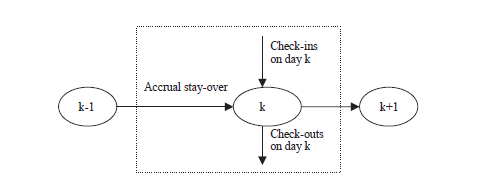
\includegraphics{Figure1.PNG}
  \caption{Flujo de check-ins y check-outs para el día k.}
  \label{fig:Figure2.1}
\end{figure}

La siguiente ecuaci{on modela la ocupaci{on del hotel para el día $k$ con $k = 1,2,3,...,(T-1)$:$$\sum_{i=0}^{k-1}\sum_{j=k+1}^{T} x_{i,j} + \sum_{j=k+1}^{T} x_{k,j} - \sum_{i=0}^{k-1} x_{i,k}$$

Debemos considerar también que el hotel tiene una capacidad limitada, por lo tanto se tienen las siguientes restricciones para el día $k$:
$$\sum_{i=0}^{k-1}\sum_{j=k+1}^{T} x_{i,j} + \sum_{j=k+1}^{T} x_{k,j} - \sum_{i=0}^{k-1} x_{i,k} \leq C$$

Para el día 0, se asume que no hay \emph{check-outs} ni estancias que crucen a ese día, de tal forma que se tiene la siguiente ecuación para el día 0: 
$$\sum_{j=1}^{T} x_{0,j} \leq C$$

El modelo de optimización se define como sigue:

Maximizar: $$\sum_{i=0}^{T-1}\sum_{j=i+1}^{T} R_{i,j}x_{i,j}$$

Sujeto a: $$\sum_{i=0}^{k-1}\sum_{j=k+1}^{T} x_{i,j} + \sum_{j=k+1}^{T} x_{k,j} - \sum_{i=0}^{k-1} x_{i,k} \leq C$$
$$\sum_{j=1}^{T} x_{0,j} \leq C$$
$$x_{i,j} \leq U_{i,j}$$
$$x_{i,j} \geq 0$$
$$\forall 0\leq i < j \leq T$$

Si bien este problema pareciera ser un problema de integración lineal, se debe considerar que los parámetros $U_{i,j}$ son desconocidos al inicio del periodo de planeación. Mas aún, los ingresos pudieran no ser fijos como se quisiera ya que recordemos que se pueden fijar distintos precios para la misma habitación, lo que puede resultar en una variación de la demanda del producto. Una manera de resolver este problema pudiera ser reemplazando los parámetros por su mejor estimador puntual, en primera instancia utilizando la esperanza de $E(U_{i,j})$.

Muchas veces utilizando este método se pueden obtener resultados razonables, sin embargo esto no siempre garantiza una solución factible y para solucionar esto se han utilizado otras herramientas como la \emph{Optimización Robusta} que es un enfoque proactivo usado para resolver problemas estocásticos.

\subsection*{Resumen}

Los modelos de optimización de ingresos han tenido un gran avance en la industria de las aerolíneas, sin embargo, aún hay un trecho muy largo por recorrer para poder aplicarlos con el mismo nível de maduréz en la industria de la hotelería.

Como se revisó anteriormente, existen muchas propuestas de enfoques diferentes para la implementación del modelo de optimización de ingresos en hoteles y la elección de alguno de ellos dependerá de los siguientes factores:

\begin{itemize}
  \item Habilidades estadísticas del equipo administrativo de la propiedad
  \item Nível de desagregación de datos con los que cuenta la propiedad
  \item Capacidad de cómputo con el que la propiedad cuenta para el cálculo del modelo
  \item Nível de automatización de procesos dentro de la propiedad, es decir, si cuenta con la capacidad de poder hacer cambios de precios e inventarios en línea
\end{itemize}

Si bien, en el apartado anterior se presentaron enfoques de vanguardia (modelos de inteligencia artificial y modelos de big data) que toman en cuenta toda la información generada por los sistemas propios del hotel y fuentes externas para ser procesado por un modelo de \emph{caja negra} para obtener un resultado, este tipo de modelos no permiten que el equipo que lo opera comprendan plenamente su funcionamiento, lo cual censura las aportaciones que el equipo pueda hacer para enriquecerlo, es por ello que para fines de este trabajo de investigación utilizaremos un modelo convencional compuesto por dos módulos: un módelo de regresión poisson para el cálculo del pronóstico de la demanda, y un módelo de maximización sujeto a restricciones para el cálculo de precios óptimos por día de reservación.

El primer módulo pronósticará la demanda utilizando datos para un hotel de negocios ubicado en una de las avenidas más importantes de la Ciudad de México. El set de datos con el que se contó durante esta investigación contenía el detalle de cada una de las reservaciones realizadas para esta propiedad desde 2014 hasta el 11 de agosto de 2018.

El segundo módulo asignará los precios óptimos para un tipo de habitación estándar tomando en cuenta los días de antelación con los que se reserva una habitación en la propiedad, de tal forma que al finalizar el proceso se cuente con una matriz de días de antelación vs precio óptimo.

En los apartados posteriores se explicará a detalle la construcción del módelo propuesto y los resultados obtenidos.